\chapter{Resultados Econométricos Iniciais}
\label{chap:resultados_ols}

Este capítulo apresenta os primeiros resultados econométricos da dissertação,
obtidos a partir de modelos lineares estimados por mínimos quadrados ordinários
(OLS). O objetivo central é avaliar empiricamente se o prêmio de risco de
volatilidade do Bitcoin (BVRP) contém informação relevante para a previsão dos
retornos futuros do ativo em diferentes horizontes temporais.

As análises desenvolvidas neste capítulo seguem diretamente o arcabouço
metodológico apresentado no Capítulo~\ref{chap:metodologia}. A inferência
estatística é conduzida com erros padrão robustos à heterocedasticidade e à
autocorrelação serial, utilizando o estimador HAC (Newey--West), garantindo
validade estatística mesmo na presença de dependência temporal nos retornos
financeiros.

Os resultados aqui apresentados devem ser interpretados como evidência empírica
inicial. Embora modelos lineares possuam capacidade limitada para capturar
não linearidades, interações complexas e mudanças de regime — características
marcantes do mercado de criptoativos —, eles fornecem uma base empírica
transparente e comparável à literatura clássica sobre prêmio de risco de
volatilidade, permitindo avaliar a direção, a magnitude e a significância
estatística do efeito associado ao BVRP.

% =========================================================
\section{Motivação e desenho empírico}
\label{sec:motivacao_ols}

A literatura sobre prêmio de risco de volatilidade documenta que a diferença
entre volatilidade implícita e volatilidade realizada reflete não apenas
expectativas sobre a incerteza futura, mas também componentes associados à
aversão ao risco, à demanda por proteção e a fricções de mercado no segmento de
derivativos. Em mercados tradicionais, há evidências consistentes de que o
prêmio de risco de volatilidade está relacionado a retornos futuros e a regimes
distintos de mercado.

No contexto do Bitcoin, essas questões tornam-se particularmente relevantes.
O mercado de criptoativos é caracterizado por elevada volatilidade estrutural,
frequentes episódios de estresse, liquidações alavancadas e participação
heterogênea de agentes. Nesse ambiente, o BVRP pode capturar variações nas
expectativas de risco e na precificação da incerteza, potencialmente
antecipando movimentos futuros dos retornos no mercado à vista.

A estratégia empírica adotada consiste em estimar regressões lineares nas quais
os retornos futuros acumulados do Bitcoin são explicados pelo BVRP observado no
tempo $t$. As estimações são realizadas para múltiplos horizontes de previsão,
permitindo investigar se o conteúdo informacional do prêmio de risco de
volatilidade se manifesta de forma distinta ao longo do tempo.

Todas as especificações respeitam estritamente a ordenação temporal dos dados,
evitando viés de \textit{look-ahead}. O BVRP é sempre medido no tempo $t$, enquanto
os retornos correspondem a períodos futuros, assegurando que apenas informação
disponível \textit{ex ante} seja utilizada na análise.

% =========================================================
\section{Resultados OLS univariados}
\label{sec:ols_univariado}

Nesta seção são apresentados os resultados das regressões OLS univariadas, cujo
objetivo é avaliar a relação empírica entre o prêmio de risco de volatilidade do
Bitcoin (BVRP) e os retornos futuros do ativo em diferentes horizontes temporais.
A inferência estatística é conduzida com erros padrão robustos à
heterocedasticidade e autocorrelação, utilizando o estimador HAC de
Newey--West.

O modelo estimado é dado por:
\begin{equation}
R_{t+h} = \alpha_h + \beta_h \cdot \text{BVRP}_t + \varepsilon_{t+h},
\end{equation}
em que $R_{t+h}$ representa o retorno futuro acumulado do Bitcoin no horizonte
$h$ dias à frente e $\text{BVRP}_t$ corresponde ao prêmio de risco de
volatilidade observado no tempo $t$.

A Tabela~\ref{tab:ols_basico_multihoriz} apresenta os coeficientes estimados para
múltiplos horizontes de previsão. Observa-se que o coeficiente associado ao BVRP
apresenta sinal positivo em todos os horizontes analisados, sugerindo que níveis
mais elevados do prêmio de risco de volatilidade estão associados, em média, a
retornos futuros mais altos do Bitcoin.

\IfFileExists{tables/tab_ols_basico_multihoriz.tex}{
  \begin{table}[H]
\centering
\caption{Resultados OLS (HAC) do BVRP para múltiplos horizontes.}
\label{tab:ols_basico_multihoriz}
\footnotesize
\begin{adjustbox}{max width=\textwidth}
\begin{tabular}{rrrrrr}
\toprule
horizon & beta & t\_stat & p\_value & $R^2$ & N \\
\midrule
1  & 0.001168 & 1.305558 & 0.191703 & 0.001242 & 1258 \\
5  & 0.005242 & 1.375767 & 0.168894 & 0.005224 & 1258 \\
10 & 0.010678 & 1.763776 & 0.077770 & 0.010748 & 1258 \\
20 & 0.022468 & 2.479869 & 0.013143 & 0.022140 & 1258 \\
30 & 0.035316 & 3.181264 & 0.001466 & 0.036095 & 1258 \\
60 & 0.044828 & 2.597009 & 0.009404 & 0.027337 & 1258 \\
\bottomrule
\end{tabular}
\end{adjustbox}
\end{table}

}{
  \begin{center}
  \fbox{\parbox{0.92\linewidth}{
  \textbf{Aviso:} arquivo \texttt{tables/tab\_ols\_basico\_multihoriz.tex} não encontrado.
  Faça upload desse arquivo para a pasta \texttt{tables/}.}}
  \end{center}
}

Em horizontes de curtíssimo prazo, a relação estimada tende a ser mais fraca e,
em geral, estatisticamente indistinguível de zero, consistente com a presença
de ruído microestrutural e choques idiossincráticos. Para horizontes
intermediários, em especial entre 20 e 30 dias, a evidência torna-se mais
robusta, em linha com a interpretação de que a informação contida no mercado de
opções se materializa de forma gradual nos retornos do ativo subjacente.

% =========================================================
\section{Análise por horizonte temporal}
\label{sec:analise_horizontes}

Para facilitar a interpretação dos resultados multihorizonte,
a Figura~\ref{fig:beta_horizonte_basico} apresenta a trajetória do coeficiente
$\beta_h$ associado ao BVRP ao longo dos diferentes horizontes de previsão no
modelo OLS básico (HAC).

\IfFileExists{tables/fig_beta_por_horizonte_basico.tex}{
  % Auto-gerado pelo notebook
\begin{figure}[!htbp]
    \centering
    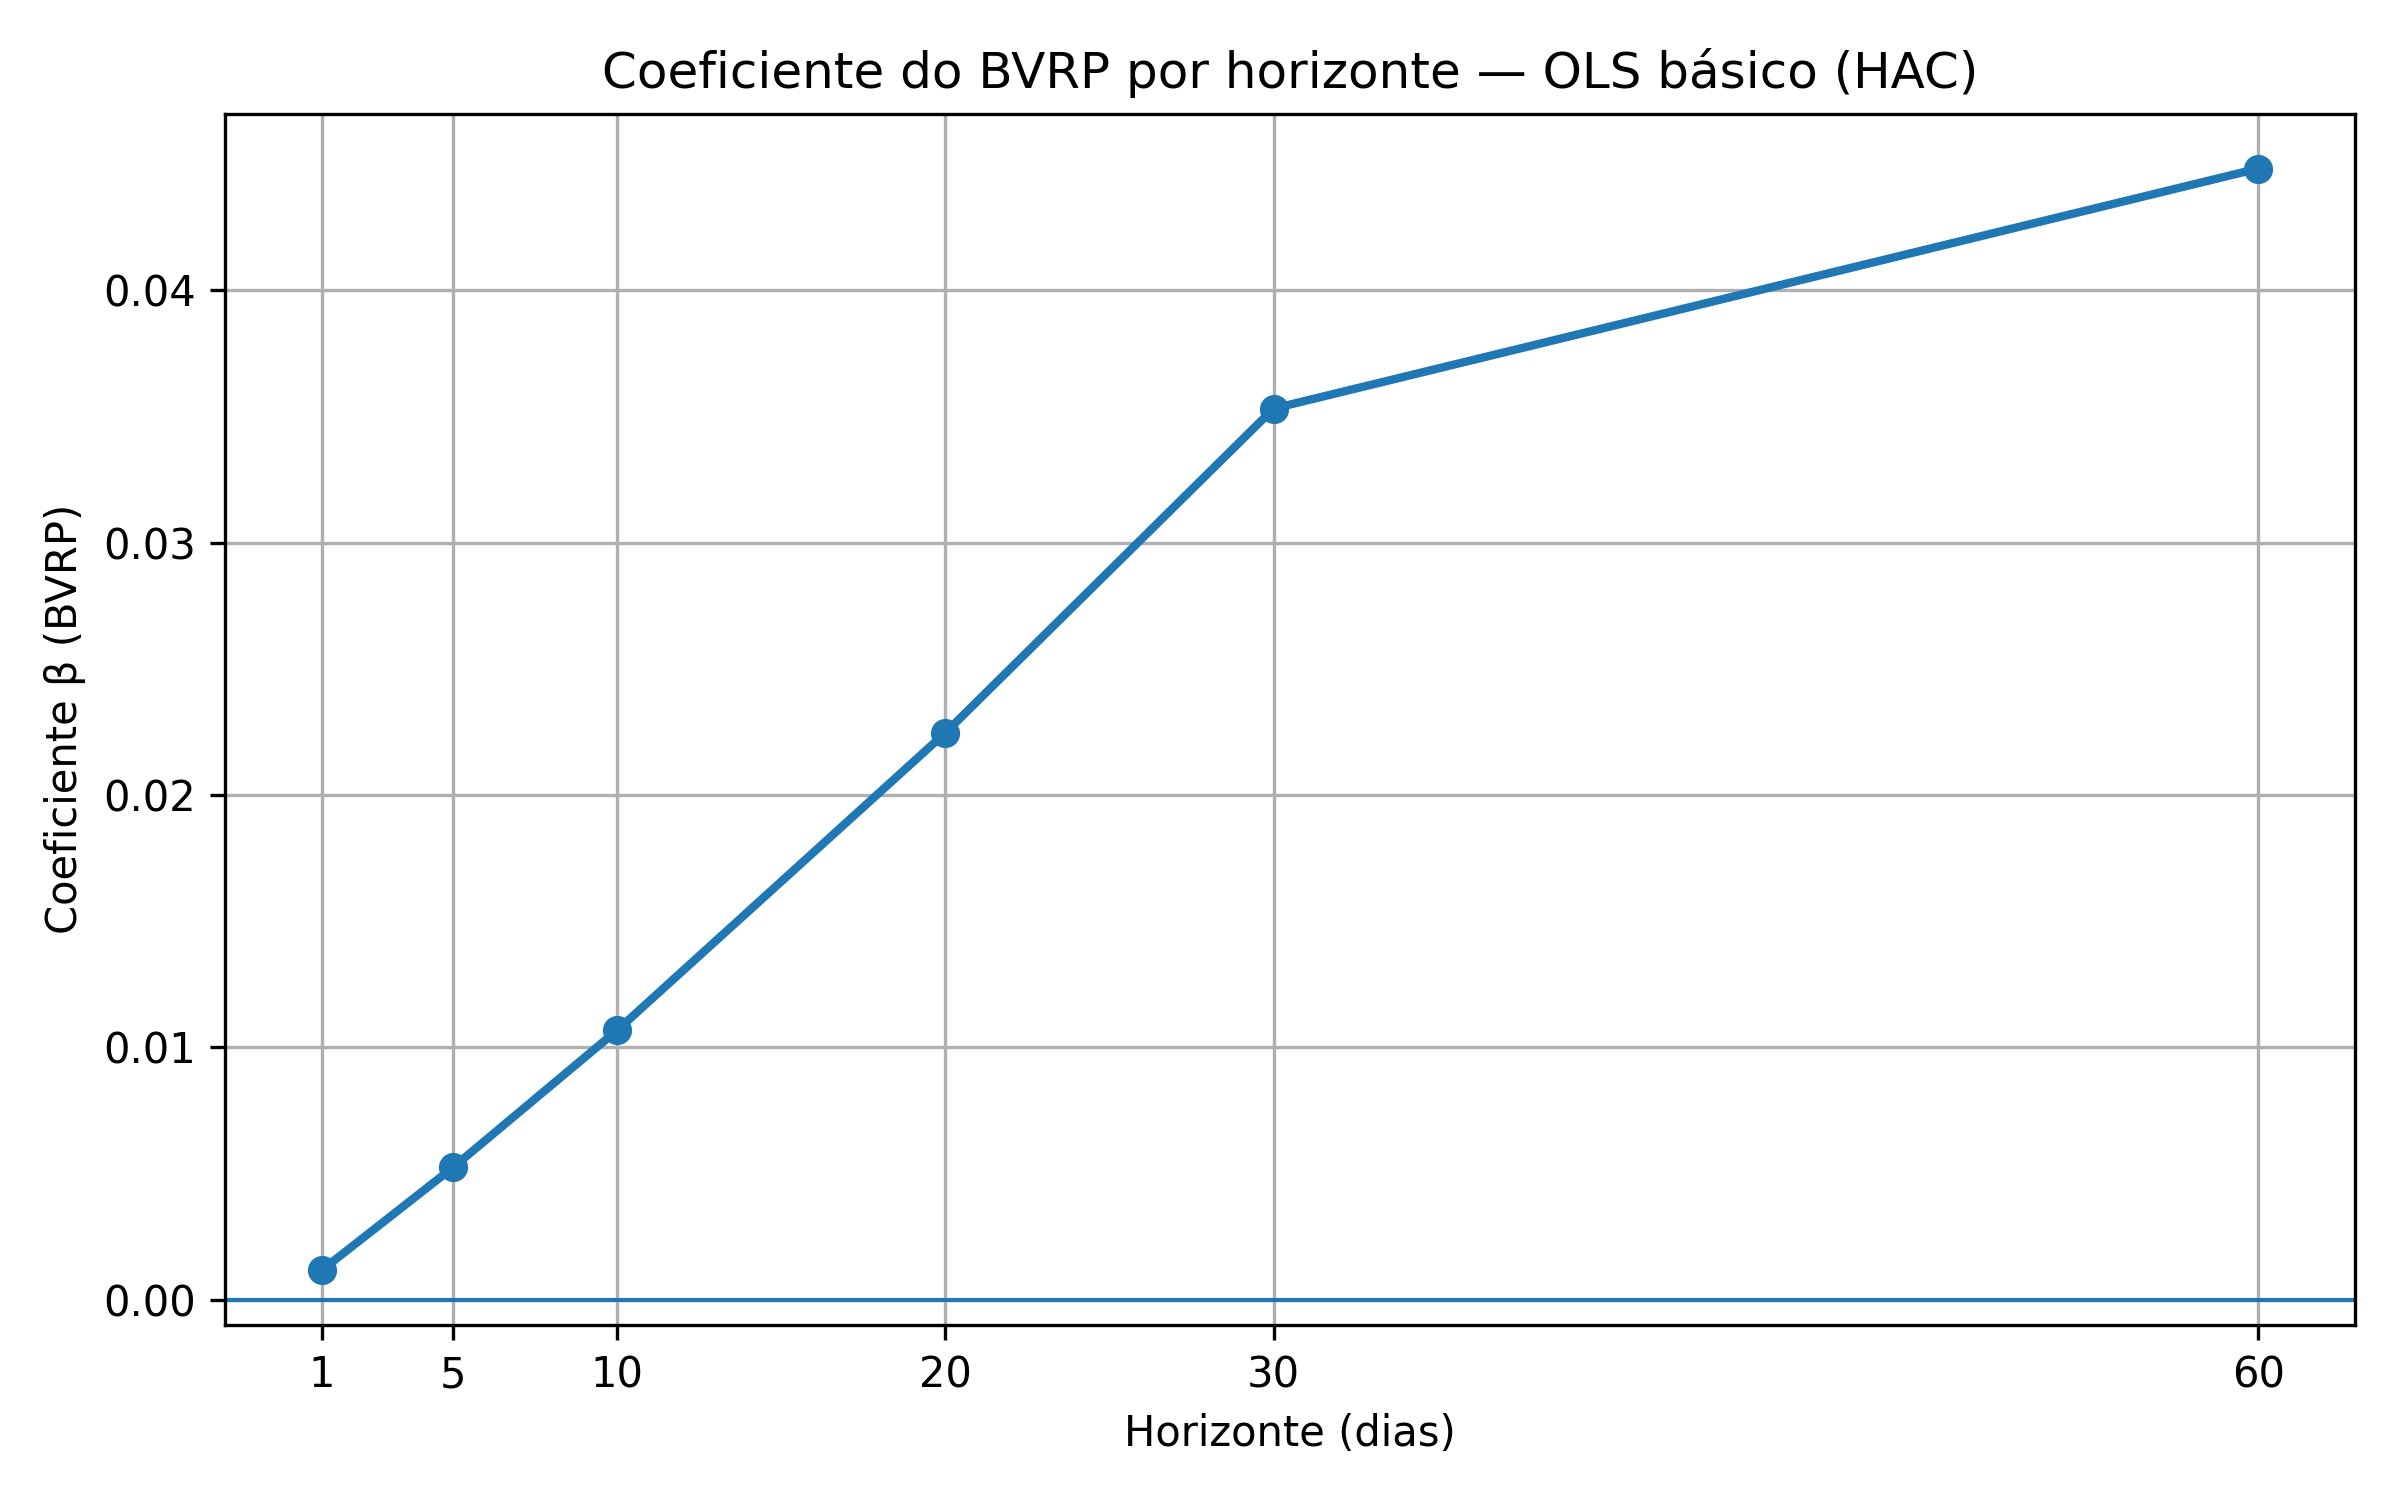
\includegraphics[width=0.85\textwidth]{figs/fig_beta_por_horizonte_basico.png}
    \caption{Coeficiente estimado do BVRP em regressões OLS (HAC) para diferentes horizontes de previsão.}
    \label{fig:beta_horizonte_basico}
\end{figure}

}{
  \begin{center}
  \fbox{\parbox{0.92\linewidth}{
  \textbf{Aviso:} arquivo \texttt{tables/fig\_beta\_por\_horizonte\_basico.tex} não encontrado.
  Faça upload desse arquivo para a pasta \texttt{tables/}.}}
  \end{center}
}

A análise evidencia que a magnitude do coeficiente do BVRP tende a aumentar à
medida que o horizonte de previsão se alonga, atingindo valores mais elevados
em janelas intermediárias. Esse padrão sugere que o conteúdo informacional do
prêmio de risco de volatilidade não se manifesta de forma imediata nos retornos
de curtíssimo prazo, mas se incorpora aos preços de maneira mais clara ao longo
do tempo.

% =========================================================
\section{Diagnóstico visual}
\label{sec:diagnostico_visual}

Como complemento à análise quantitativa, a
Figura~\ref{fig:scatter_bvrp_ret_30d} apresenta o gráfico de dispersão entre o
BVRP observado no tempo $t$ e o retorno futuro acumulado do Bitcoin no horizonte
de 30 dias, juntamente com a reta estimada via OLS.

\IfFileExists{tables/fig_scatter_bvrp_ret_fut_30d.tex}{
  % Auto-gerado pelo notebook
\begin{figure}[!htbp]
    \centering
    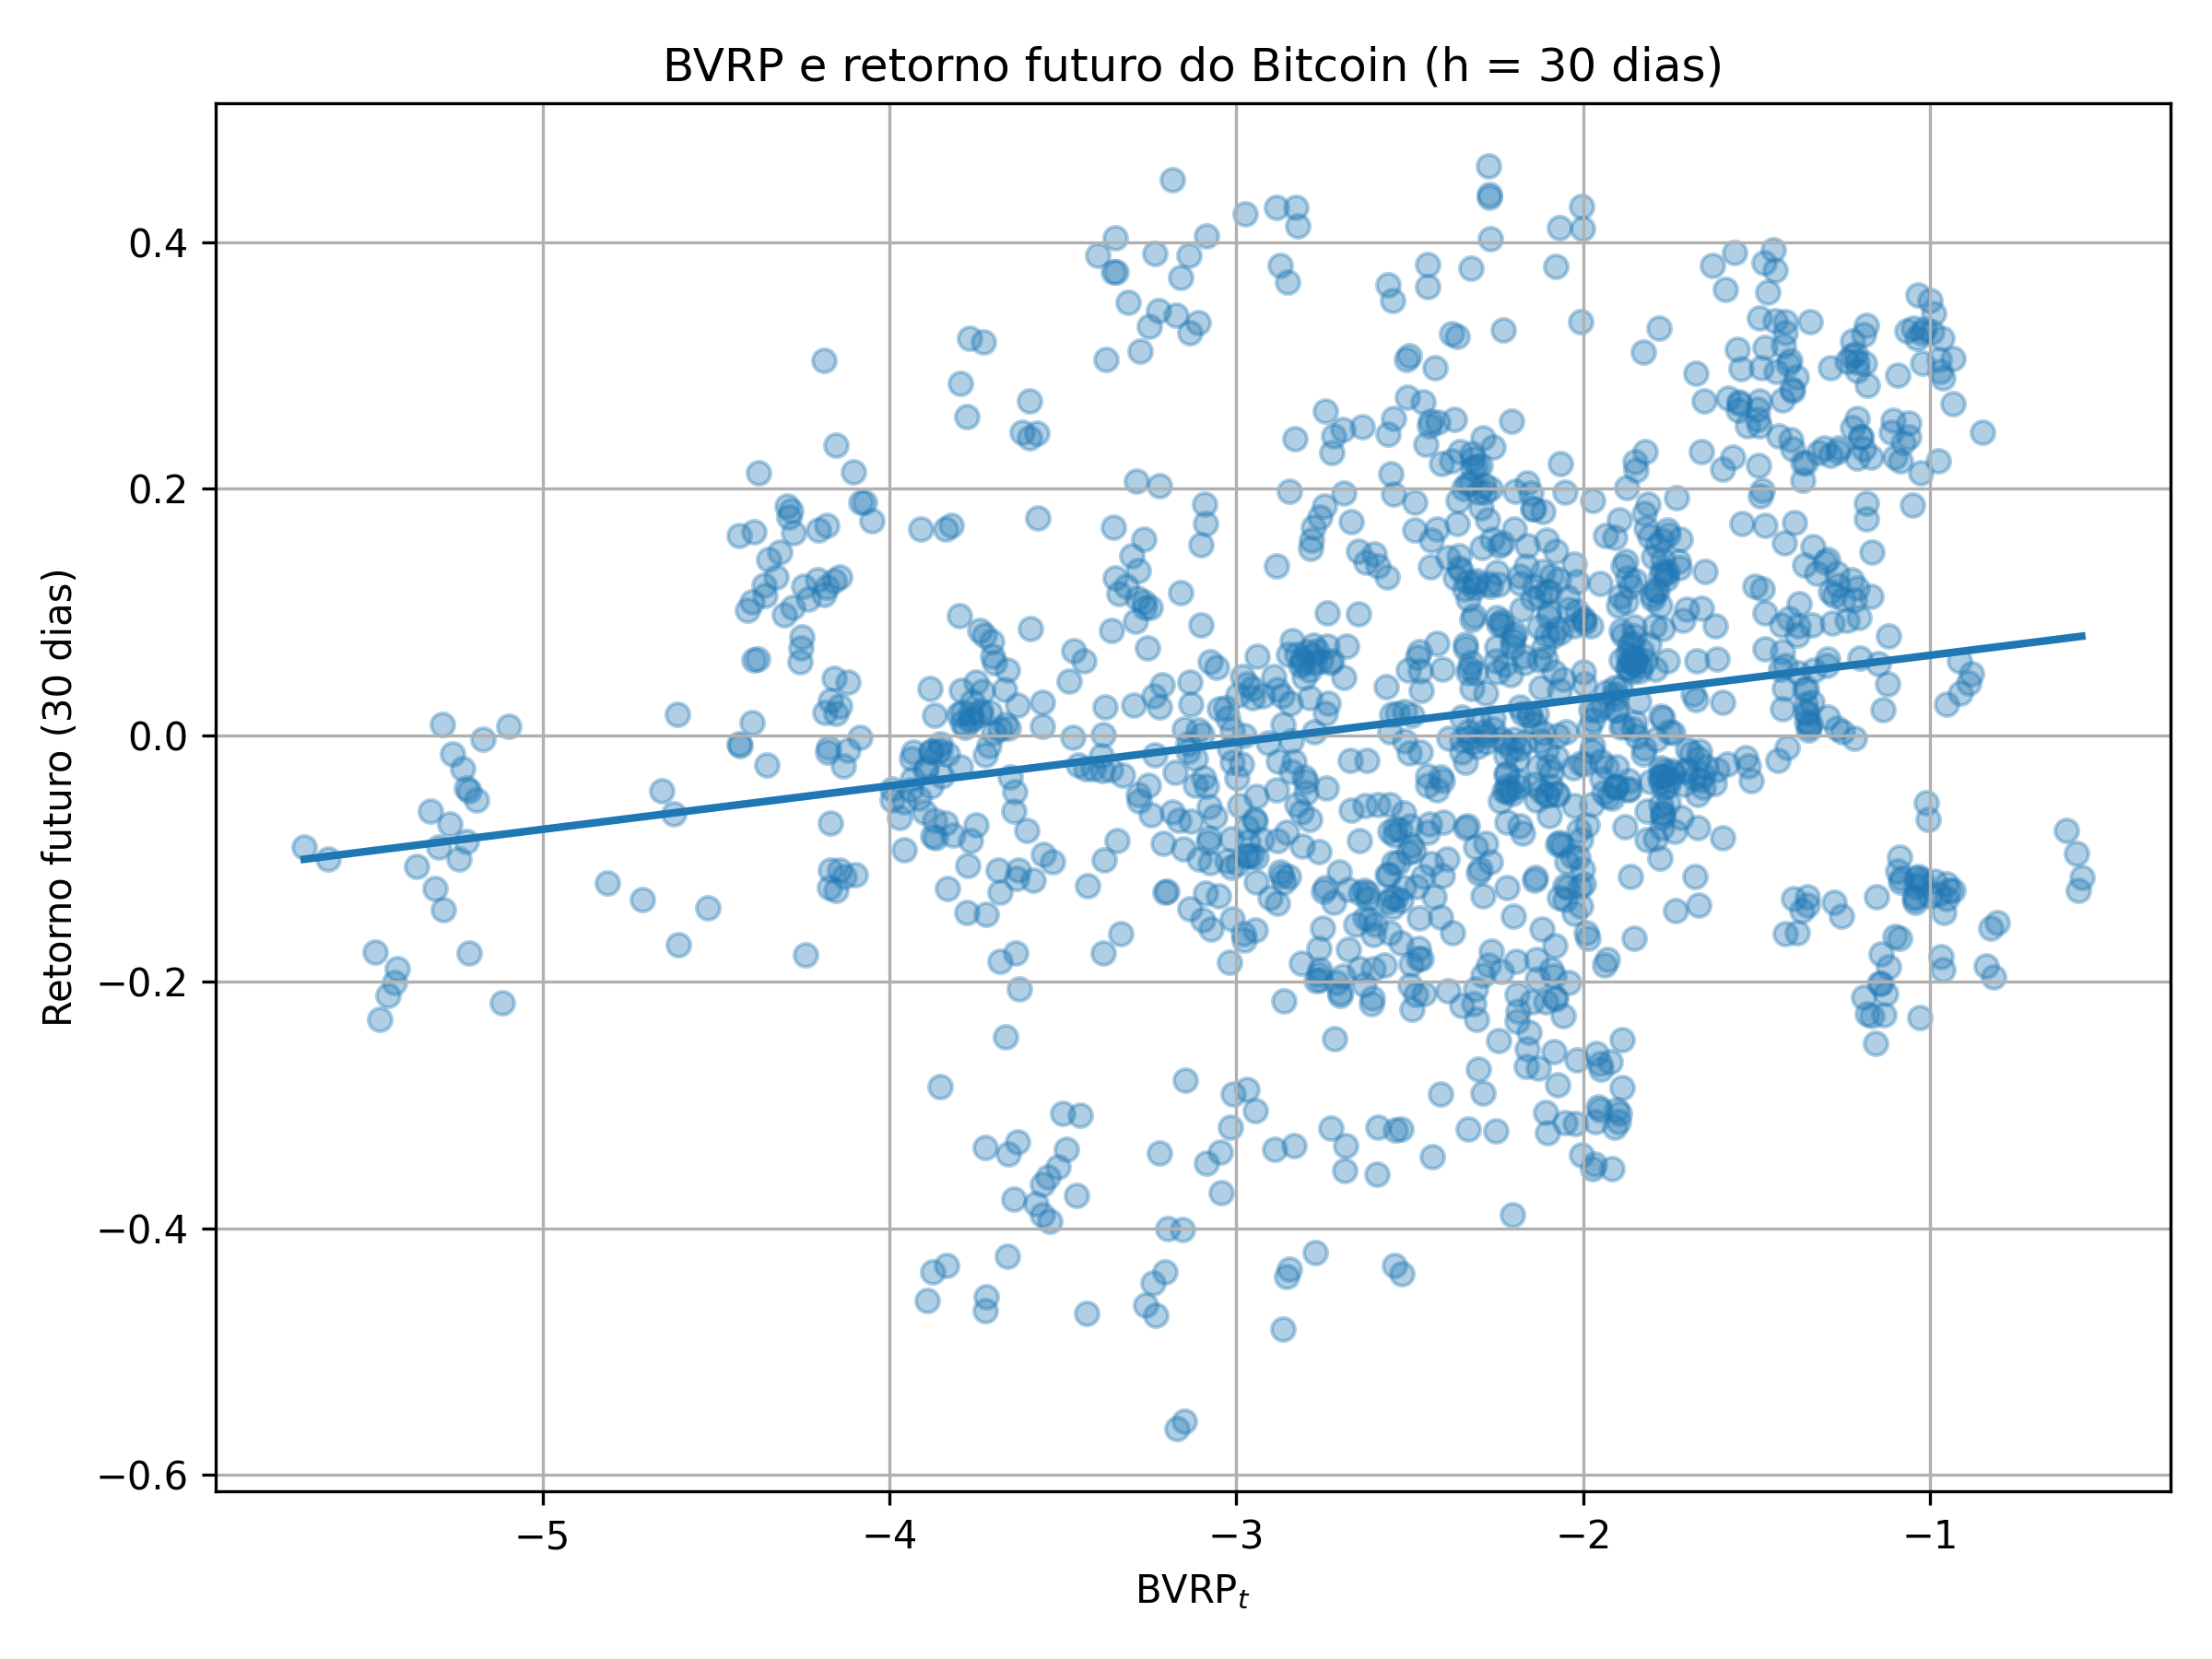
\includegraphics[width=0.85\textwidth]{figs/fig_scatter_bvrp_ret_fut_30d.png}
    \caption{Dispersão entre o prêmio de risco de volatilidade do Bitcoin (BVRP) no tempo $t$ e o retorno futuro acumulado em 30 dias, com reta ajustada por OLS.}
    \label{fig:scatter_bvrp_ret30}
\end{figure}

}{
  \begin{center}
  \fbox{\parbox{0.92\linewidth}{
  \textbf{Aviso:} arquivo \texttt{tables/fig\_scatter\_bvrp\_ret\_fut\_30d.tex} não encontrado.
  Faça upload desse arquivo para a pasta \texttt{tables/}.}}
  \end{center}
}

O gráfico sugere uma relação média positiva entre o prêmio de risco de
volatilidade e os retornos futuros, embora acompanhada por elevada dispersão —
característica típica do mercado de criptoativos, no qual choques exógenos,
mudanças de regime e eventos extremos desempenham papel relevante na dinâmica
dos preços.

% =========================================================
\section{Robustez com controles de volatilidade}
\label{sec:robustez_ols}

Para avaliar a robustez dos resultados, a especificação básica é estendida de
modo a incluir controles explícitos para volatilidade realizada e volatilidade
implícita:
\begin{equation}
R_{t+h} = \alpha_h
+ \beta_{1,h}\cdot \text{BVRP}_t
+ \beta_{2,h}\cdot \text{RV}_t
+ \beta_{3,h}\cdot \text{IV}_t
+ \varepsilon_{t+h}.
\end{equation}

A Tabela~\ref{tab:ols_controles_multihoriz} reporta os resultados para múltiplos
horizontes de previsão.

\IfFileExists{tables/tab_ols_controles_multihoriz.tex}{
  \begin{table}[H]
\centering
\caption{Resultados OLS (HAC) com controles de volatilidade (RV e IV) para múltiplos horizontes.}
\label{tab:ols_controles_multihoriz}
\footnotesize
\begin{adjustbox}{max width=\textwidth}
\begin{tabular}{rrrrrrrr}
\toprule
horizon & beta\_BVRP & t\_BVRP & p\_BVRP & beta\_RV & beta\_IV & $R^2$ & N \\
\midrule
1  & 0.002500  &  0.858364 & 0.390691 &  0.000773 &  0.003273 & 0.001547 & 1258 \\
5  & -0.000544 & -0.052644 & 0.958016 & -0.004475 & -0.005019 & 0.005575 & 1258 \\
10 & -0.008631 & -0.550320 & 0.582100 & -0.014198 & -0.022829 & 0.013391 & 1258 \\
20 & -0.026950 & -1.145006 & 0.252207 & -0.035810 & -0.062760 & 0.030858 & 1258 \\
30 & -0.046138 & -1.500763 & 0.133417 & -0.058840 & -0.104977 & 0.051983 & 1258 \\
60 & -0.106881 & -2.150230 & 0.031537 & -0.107324 & -0.214205 & 0.056107 & 1258 \\
\bottomrule
\end{tabular}
\end{adjustbox}
\end{table}

}{
  \begin{center}
  \fbox{\parbox{0.92\linewidth}{
  \textbf{Aviso:} arquivo \texttt{tables/tab\_ols\_controles\_multihoriz.tex} não encontrado.
  Faça upload desse arquivo para a pasta \texttt{tables/}.}}
  \end{center}
}

A Figura~\ref{fig:beta_comparacao_basico_controles} compara, por horizonte, o
coeficiente do BVRP estimado no modelo básico e no modelo com controles (HAC).

\IfFileExists{tables/fig_beta_comparacao_basico_vs_controles.tex}{
  % Auto-gerado pelo notebook
\begin{figure}[!htbp]
    \centering
    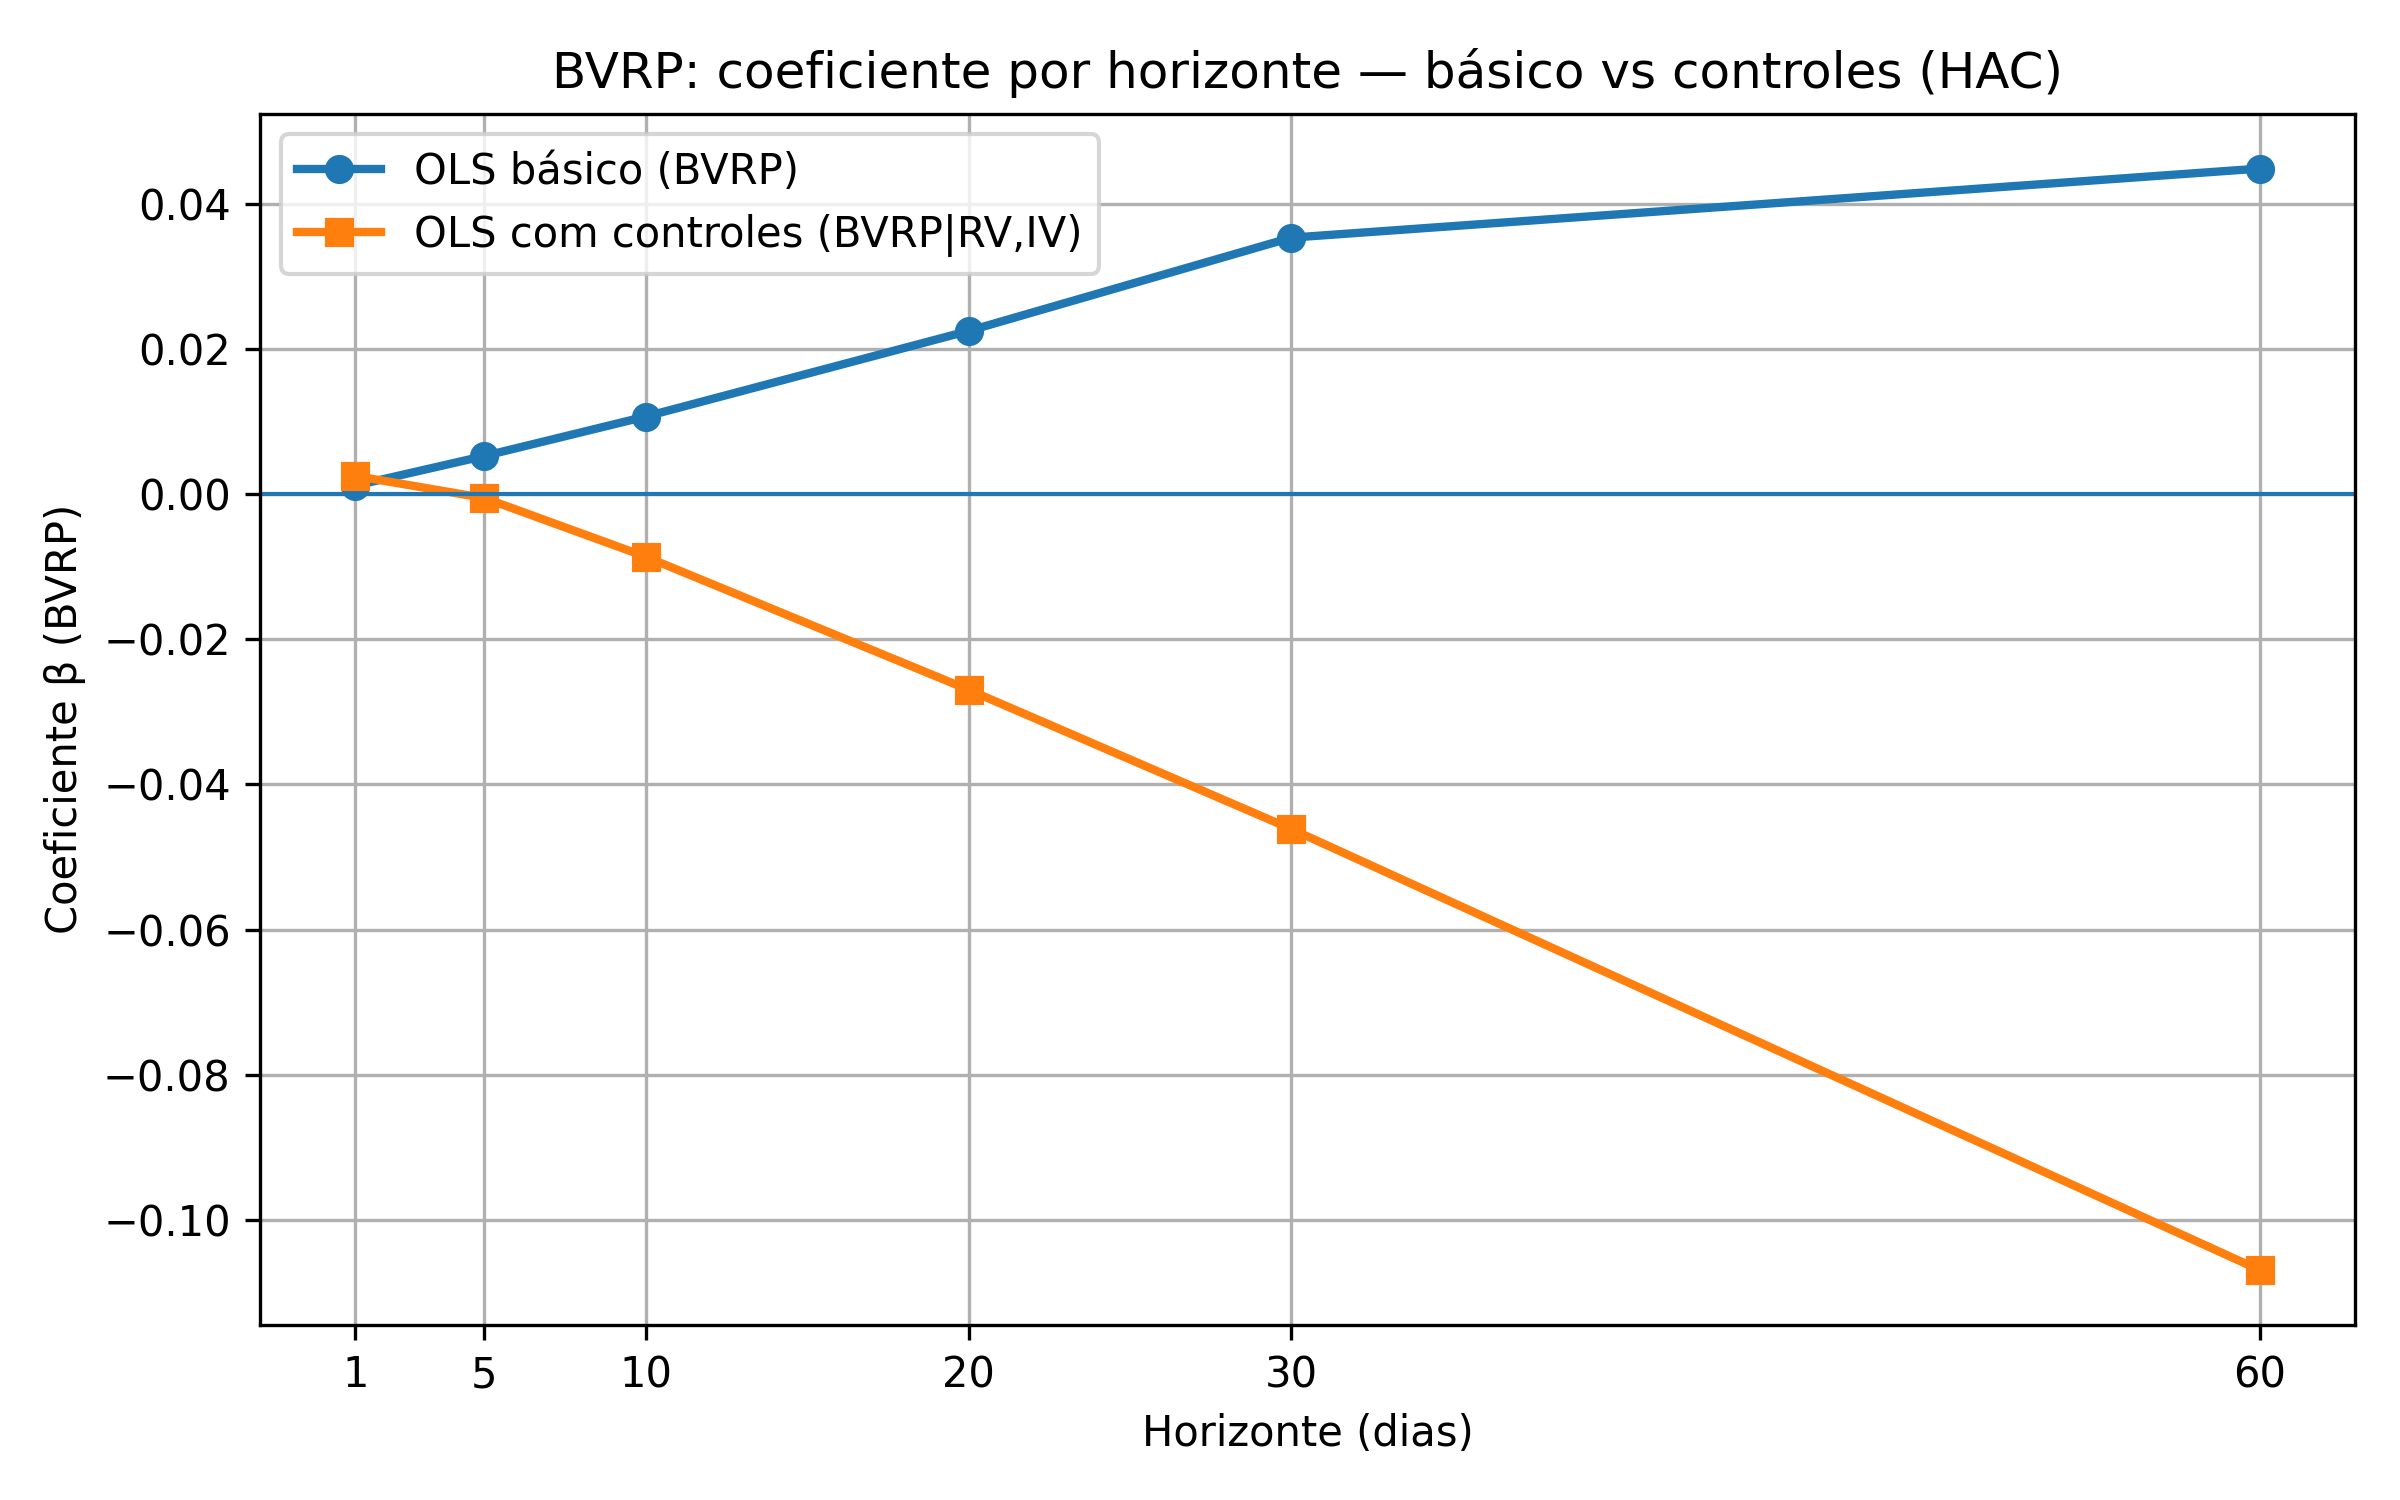
\includegraphics[width=0.85\textwidth]{figs/fig_beta_comparacao_basico_vs_controles.png}
    \caption{Comparação do coeficiente do BVRP entre o modelo OLS básico e o modelo com controles de volatilidade (RV e IV), ao longo de diferentes horizontes de previsão.}
    \label{fig:beta_comparacao_basico_controles}
\end{figure}

}{
  \begin{center}
  \fbox{\parbox{0.92\linewidth}{
  \textbf{Aviso:} arquivo \texttt{tables/fig\_beta\_comparacao\_basico\_vs\_controles.tex} não encontrado.
  Faça upload desse arquivo para a pasta \texttt{tables/}.}}
  \end{center}
}

De modo geral, a inclusão simultânea de IV e RV reduz a significância estatística
do coeficiente associado ao BVRP em alguns horizontes, refletindo a elevada
correlação entre as variáveis explicativas, dado que o BVRP é definido como uma
diferença entre IV e RV. Assim, a evidência deve ser interpretada com cautela:
a contribuição marginal do BVRP em modelos lineares aditivos pode ser atenuada
por multicolinearidade, mesmo que a variável continue capturando condições
agregadas de risco precificadas no mercado de opções.

% =========================================================
\section{Síntese dos resultados}
\label{sec:sintese_ols}

Em conjunto, os resultados deste capítulo fornecem evidência empírica inicial
de que o prêmio de risco de volatilidade do Bitcoin contém informação relevante
para a previsão de retornos futuros, sobretudo em horizontes de médio prazo.
Embora o poder explicativo dos modelos lineares seja limitado, os coeficientes
estimados apresentam sinais consistentes com a interpretação econômica do BVRP.

A análise de robustez sugere que parte do efeito identificado é mediada pelo
nível geral de volatilidade do mercado e que a relação pode envolver
não linearidades, interações e efeitos de regime. Esses aspectos motivam a
análise desenvolvida no capítulo seguinte, no qual são empregadas técnicas de
aprendizado de máquina para capturar padrões mais complexos na relação entre o
BVRP e os retornos futuros do Bitcoin.
